\documentclass[12pt]{exam}

\usepackage{tikz} % Used for Groupwork 7 PHP

% essential packages
\usepackage{fullpage} % margin formatting
\usepackage{enumitem} % configure enumerate and itemize
\usepackage{amsmath, amsfonts, amssymb, mathtools} % math symbols
\usepackage{xcolor, colortbl} % colors, including in tables
\usepackage{makecell} % thicker \Xhline in table
\usepackage{graphicx} % images, resizing

% sometimes needed packages
\usepackage{hyperref} % hyperlinks
% \hypersetup{colorlinks=true, urlcolor=blue}
% \usepackage{logicproof} % natural deduction
% \usepackage{tikz} % drawing graphs
% \usetikzlibrary{positioning}
% \usepackage{multicol}
% \usepackage{algpseudocode} % pseudocode

% paragraph formatting
\setlength{\parskip}{6pt}
\setlength{\parindent}{0cm}

% newline after Solution:
\renewcommand{\solutiontitle}{\noindent\textbf{Solution:}\par\noindent}

% less space before itemize/enumerate
\setlist{topsep=0pt}

% creates \filcl to grey out cells for groupwork grading
\newcommand{\filcl}{\cellcolor{gray!25}}

% creates \probnum to get the problem number
\newcounter{probnumcount}
\setcounter{probnumcount}{1}
\newcommand{\probnum}{\arabic{probnumcount}. \addtocounter{probnumcount}{1}}

% use roman numerals by default
\setlist[enumerate]{label={(\roman*)}}

% creates custom list environments for grading guidelines, question parts
\newlist{guidelines}{itemize}{1}
\setlist[guidelines]{label={}, left=0pt .. \parindent, nosep}
\newlist{gwguidelines}{enumerate}{1}
\setlist[gwguidelines]{label={(\roman*)}, nosep}
\newlist{qparts}{enumerate}{2}
\setlist[qparts]{label={(\alph*)}}
\newlist{qsubparts}{enumerate}{2}
\setlist[qsubparts]{label={(\roman*)}}
\newlist{stmts}{enumerate}{1}
\setlist[stmts]{label={(\roman*)}, nosep}
\newlist{pflist}{itemize}{4}
\setlist[pflist]{label={$\bullet$}, nosep}
\newlist{enumpflist}{enumerate}{4}
\setlist[enumpflist]{label={(\arabic*)}, nosep}

\printanswers

\newcommand{\prevhwnum}{6}
\newcommand{\hwnum}{7}

\begin{document}
\setcounter{probnumcount}{1}
\section*{Groupwork \hwnum{} Problems}


\subsection*{\probnum Get to the Point [10 points]}
Consider an arbitrary set $A$. We say a function $f:A\rightarrow A$ has a \textit{fixed point} iff there exists $a \in A$ such that $f(a) = a$.

Consider the notation $f^{(n)}$ to mean $\underbrace{f \circ \dots \circ f}_{n \text{ times}}$, where $n \in \mathbb{Z^+}$. Essentially, $n$ copies of $f$ are composed together.

Prove by \textbf{induction} that if $f$ is a function with a fixed point, then for all positive integers $n$, $f^{(n)}$ has a fixed point.

\begin{solution}
	% function $f:A\rightarrow A$ has a fixed point $\iff$ there exists $a \in A$ such that $f(a) = a$.\\
	Let P(n) be the statement that $f^{(n)}$ has a fixed point.\\
	Inductive step: Assume P(k) is true for some $k \in \mathbb{Z^+}$. \\
	Want to show: $P(k) \implies P(k+1)$ for all $k \in \mathbb{Z^+}$.\\
	i.e. $\exists a \in A$ such that $f^{(k)}(a) = a \implies \exists b \in A$ such that $f^{(k+1)}(b) = b$.\\
	$f^{(k+1)}(b) = f(f^{(k)}(b))$.\\
	By inductive hypothesis, $f^{(k)}(b) = b$.\\
	Then $f(f^{(k)}(b)) = f(b) = b$.\\
	So $b$ is a fixed point of $f^{(k+1)}$.\\
	Thus, $P(k) \implies P(k+1)$ for all $k \in \mathbb{Z^+}$.\\
	Base case: $n=1$. Then $f^{(1)} = f$ has a fixed point by assumption.
\end{solution}


\subsection*{\probnum Going Off the Grid [8 points]}
In a grid, we say that a point $a$ \textit{dominates} a point $b$ iff $a$ lies strictly above and to the right of $b$. For example, in the picture below, $a$ dominates $b$.
\begin{center}
	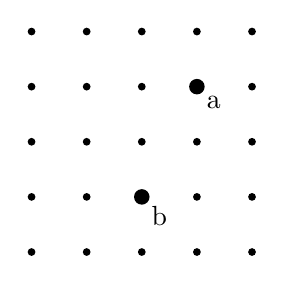
\begin{tikzpicture}[scale=0.7]
		\def\n{5}
		\foreach \x in {1,...,\n} {
				\foreach \y in {1,...,\n} {
						\ifnum\x=3
							\ifnum\y=2
								\fill (\x,\y) circle (4pt);
								\node[anchor=north west] at (\x,\y) {b};
							\else
								\fill (\x,\y) circle (2pt);
							\fi
						\else
							\ifnum\x=4
								\ifnum\y=4
									\fill (\x,\y) circle (4pt);
									\node[anchor=north west] at (\x,\y) {a};
								\else
									\fill (\x,\y) circle (2pt);
								\fi
							\else
								\fill (\x,\y) circle (2pt);
							\fi
						\fi
					}
			}
	\end{tikzpicture}
\end{center}
Prove using the Pigeonhole Principle that if we choose $4n-1$ points from an $n \times n$ grid ($n\ge 4$), there must be three chosen points $x, y, z$ such that $x$ dominates $y$ and $y$ dominates $z$. Make sure to state what your pigeons are and what your holes are, as well as how many of each you have.

\textbf{Hint:} If $x, y, z$ lie on the same increasing diagonal as shown in the picture below, then $x$ dominates $y$ and $y$ dominates $z$.
\begin{center}
	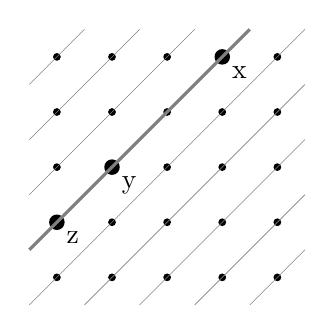
\begin{tikzpicture}[scale=0.7]
		\def\n{5}
		\foreach \x in {1,...,\n} {
				\foreach \y in {1,...,\n} {
						\ifnum\x=4
							\ifnum\y=5
								\fill (\x,\y) circle (4pt);
								\node[anchor=north west] at (\x,\y) {x};
							\else
								\fill (\x,\y) circle (2pt);
							\fi
						\else
							\ifnum\x=2
								\ifnum\y=3
									\fill (\x,\y) circle (4pt);
									\node[anchor=north west] at (\x,\y) {y};
								\else
									\fill (\x,\y) circle (2pt);
								\fi
							\else
								\ifnum\x=1
									\ifnum\y=2
										\fill (\x,\y) circle (4pt);
										\node[anchor=north west] at (\x,\y) {z};
									\else
										\fill (\x,\y) circle (2pt);
									\fi
								\else
									\fill (\x,\y) circle (2pt);
								\fi
							\fi
						\fi
					}
			}


		\draw [very thin, gray] (0.5, 4.5) -- (1.5, 5.5);
		\draw [very thin, gray] (0.5, 3.5) -- (2.5, 5.5);
		\draw [very thin, gray] (0.5, 2.5) -- (3.5, 5.5);
		\draw [very thick, gray] (0.5, 1.5) -- (4.5, 5.5);
		\draw [very thin, gray] (0.5, 0.5) -- (5.5, 5.5);
		\draw [very thin, gray] (1.5, 0.5) -- (5.5, 4.5);
		\draw [very thin, gray] (2.5, 0.5) -- (5.5, 3.5);
		\draw [very thin, gray] (3.5, 0.5) -- (5.5, 2.5);
		\draw [very thin, gray] (4.5, 0.5) -- (5.5, 1.5);

	\end{tikzpicture}
\end{center}

\begin{solution}
	Pigeons: the $4n-1$ points chosen from the grid.\\
	Holes: the $n-1$ increasing diagonals of the grid.\\
	Each point lies on exactly one increasing diagonal.\\
	By the Pigeonhole Principle, at least one increasing diagonal contains at least $\lceil \frac{4n-1}{n-1} \rceil = 4$ points.\\
	By the hint, there must be three chosen points $x, y, z$ such that $x$ dominates $y$ and $y$ dominates $z$.
	Thus, if we choose $4n-1$ points from an $n \times n$ grid ($n\ge 4$), there must be three chosen points $x, y, z$ such that $x$ dominates $y$ and $y$ dominates $z$.
\end{solution}

\end{document}
